% Chapter 4
\chapter{A WSN with Waspmotes: Implementation aspects} % Main chapter title
\label{Chapter4} % For referencing the chapter elsewhere, use \ref{Chapter1} 
\lhead{Chapter 4. \emph{A WSN with Waspmotes: Implementation aspects}}
%\textsl{Written by Frederik De Greef}
%----------------------------------------------------------------------------------------
\section{Overdrive}

for the practical part: memory (SRAM) problems:  using  = freeMemory();
Joe is true. V11 API wastes a lot of memory including always all libraries despite of you are not using them.

Try to remove every class you do not use, and also there are some certain cases that you have to remove the usage of some constants and functions.

just go one by one to the compiler msgs. We can help you if you are not sure removing something.

Regards
I'm experiencing similar problems with my Waspmotes due to other issues, a recomendation is to remove from the API library, all that classes that you don't use such as SD .h and .cpp, or GPS, etc. bear in mind that you have to remove any reference from the file WaspClasses and where the compilator throws you an exception.

XCTU problems (cannot read / reset / writes always)  cannot change device role via Libelium
  
\subsection{Device start-up}
Whether we come out of a hardware reset or a hibernate reset, the first thing the node will do is try to establish a connection with the network. Depending which reset we come from different routines will be executed. In normal operation mode this process only takes about 2 seconds (Please see appendix \ref{fig:envA} for more measurement results). However, when a node is not able to join a network it will go into panic mode. This means that if the operating sleeping time is small, this time will be ignored and the node will wake up less frequently until it is able to rejoin the network, that way saving battery power. Supposing the node is able to rejoin the network, it will send the number of panics it experienced to the coordinator so a network administrator can investigate of the severity of the problem.

\subsubsection{Full initialization}
When the program is executed for the first time or when a hardware reset is detected the XBee will execute a full initialization process and the RTC will be set to zero. This means the default PAN ID and possibly other user settings like node ID will be written to the XBee. After this write the XBee must be re-setted (turn the power off and back on) and only than the joining attempts can start. This means full initialization takes about 9 seconds on average. 

\subsubsection{Reduced initialization}
By not resetting the PAN ID but fetching it from the XBee's memory the joining process only takes about two seconds. Unfortunately a disadvantage of this shortened setup is that the XBee is no longer able to detect if the coordinator or his parent is actually available. The program will only notices this for the first time when it is trying to send a message. If this function results in a send error the program will do a full setup routine and resend the message. If the node then fails again to send the message we can conclude that the coordinator is really off-line or that there are no joinable nodes within range. 




"Now, let's try to make a simple code which hibernates well. We recommend you to put a delay of a few seconds or a led blink before PWR.hibernate() sentence to allow removing hibernate jumper correctly."

%----------------------------------------------------------------------------------------
\section{Power savings}
\subsection{In the algorithm}
\subsection{Sleep vs. Hibernate}
Compare battery life
\subsection{Variable sleep times}
In default configuration the Waspmote will send only its battery level to the default gateway and go into hibernate mode for 15 minutes. After this the cycle repeats. However it is possible that the node has more sensors implemented and the user wishes to obtain these values at different frequencies. In that case the node will have various different sleep times. \\
The next subsections will discuss different techniques to determine those sleeping intervals. In hibernation mode the node is completely disconnected from the main battery and the program stops. This makes that all variables lose their values and must be stored in EEPROM memory if they must be known during the next cycle. Each of the next techniques present with benefits and drawbacks and since we are working with embedded systems with limited possibilities, one should also consider to limit the users options to facilitate the calculations.
\subsubsection{Calculate only the next time to sleep}
Each algorithm will have to store the individual sleep times per sensor. To support this algorithm also a copy of the original time will be saved and each time the node wakes up it will look for the smallest next time to sleep. This number will be subtracted from the other sleep times in the array. When a value becomes zero it will be restored with its original value and the cycle continues.  The following example demonstrates the process:\\
\begin{table}[!hb]
\begin{center}
\begin{tabular}[!hb]{|c|c|c|c|c|}
\hline
\textbf{Sensor[4]} & \textbf{Sensor[3]} & \textbf{Sensor[2]} & \textbf{Sensor[1]} &\textbf{Sensor[0]}\\
\hline
100  & 50 & 35 & 10 & 20\\
\hline
\end{tabular}
\caption{Individual Sensor Sleep Times in seconds}
\label{tab:sleep1}
\end{center}
\end{table}
\begin{table}[!ht]
\begin{center}
\begin{tabular}[!ht]{|c|c|c|c|c|c|c|}
\hline
\textbf{Cycle} & \textbf{Sensor[4]} & \textbf{Sensor[3]} & \textbf{Sensor[2]} & \textbf{Sensor[1]} &\textbf{Sensor[0]} & \textbf{Sleep time}\\
\hline
0 & 100 & 50 & 35 & \textbf{10} & 20 & 10\\
\hline
1 & 90 & 40 & 25 & \textbf{10} & \textbf{10} & 10\\
\hline
2 & 80 & 30 & 15 & \textbf{10} & 20 & 10\\
\hline
3 & 70 & 20 & \textbf{5} & 10 & 10 & 5\\
\hline
4 & 65 & 15 & 25 & \textbf{5} & \textbf{5} & 5\\
\hline
5 & 60 & \textbf{10} & 20 & \textbf{10} & 20 & 10\\
\hline
6 & 50 & 50 & \textbf{10} & \textbf{10} & \textbf{10} & 10\\
\hline
\end{tabular}
\caption{Example of sleep algorithm 1}
\label{tab:sleep2}
\end{center}
\end{table}
This process is fast and simple. However, the main advantage is that the node has to write to EEPROM each time it wakes up. According to Atmel the EEPROM of the ATmega1281 has an endurance of at least 100,000 write / erase cycles. The following equation indicates the problem for an interval of 10 seconds:
\begin{equation}
\frac{100000 \mathrm{writes} \cdot 10 \mathrm{s}}{60 \mathrm{s} \cdot 60 \mathrm{min} \cdot 24 \mathrm{h}}= 11,57 \: \mathrm{days} 
\label{eq:1}
\end{equation}
But the processors has 4Kbytes EEPROM on board so we don't have to write to the same place every time. Since EEPROM is written on a 'per cell' basis this can extend the lifetime. Our sensor mask can contain up to 16 values of 2 bytes. This leads to the next result:
\begin{equation}
\frac{100000 \mathrm{writes} \cdot 10 \mathrm{s} \cdot 4\mathrm{KB}}{60 \mathrm{s} \cdot 60 \mathrm{min} \cdot 24 \mathrm{h} \cdot 365\mathrm{days} \cdot 32\mathrm{B}} = 3,96\: \mathrm{years}
\end{equation}
We still must store where the data is stored but this won't cause big problems since we only have to rewrite this cell 125 times:
\begin{equation}
\frac{4\mathrm{KB}}{32\mathrm{B}} = 125 \: \mathrm{writes}
\end{equation}

\subsubsection{Calculate all next times to sleep}
Another possibility is calculate as much as possible or if maybe even all sleep times. 
\subsubsection{Limit user control}


\subsection{Overdrive function}
The overdrive effect amplifies the audio signal in a non-linear way. There are different possible schemes, we used the three layer non-linear soft saturation scheme below. The treshold value is set at 1/3, given that the input audio values are between -1 and 1. 
\[ f(x) = \left\{
\begin{array}{ll}
2x & \mbox{if $0 \leq x < \frac{1}{3}$}\\
\frac{3-(2-3x)^{2}}{3} & \mbox{if $ \frac{1}{3} \leq x < \frac{2}{3}$}\\
1 & \mbox{if $ \frac{2}{3} \leq x \leq 1$}
\end{array} \right. \]
\begin{itemize}
\item In the lower third the output is linear - multiplied by 2. for $\frac{2}{3} \leq x \leq 1$
\item In the middle third there is a non-linear (quadratic) output response
\item Above $\frac{2}{3}$ the output is set to 1. 
\end{itemize}
Image \ref{fig:over} below shows the effect of the overdrive on an audio sample shown in the time domain. The blue signal is the original, the red signal is overdriven signal. (Time on the x-axis, amplitude on the y-axis.)
\begin{figure}[htbp]
\centering
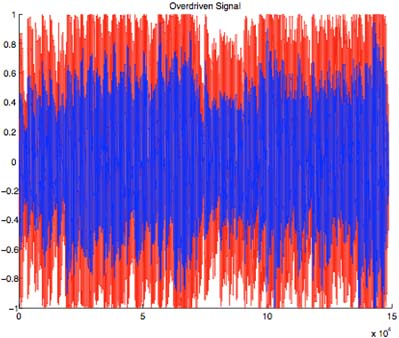
\includegraphics[height=6.5cm]{over}
\rule{30em}{0.5pt}
\caption{Effect of overdrive in time domain}
\label{fig:over}
\end{figure}
Bringing this non-linearity in the signal is called clipping. Clipping is a process that produces frequencies not originally present in the audio signal. 
These frequencies can either be ''harmonic", meaning they are whole number multiples of the signal's original frequencies, or ''inharmonic", meaning dissonant odd-order overtones. \\
Setting the treshold value also determines wich type of clipping is applied. Increasing the treshold value will result in a softer clipping. Whereas decreasing the treshold value wil result in a harder clipping. When a treshold value of 1 is defined, there is no overdrive applied. The output remains the original signal. \\ \\
The hardness or softness of the clipping matters. Hard clipping results when the output wave equals the input up/down to a certain level, then stays at the clipping level until the input drops below the clipping level again, giving perfectly flat tops and bottoms to the clipped output. Soft clipping has no abrupt clipping level, but gently rounds the top/bottom of the output wave so the waveform is "softly" rounded on top/bottom, not flat-topped.\\
Soft clipping emphasizes the lower- order harmonics, the third and fifth, etc. Hard clipping has a mix slewed to the higher order seventh and up harmonics, which are harsher sounding. \\
In the figure \ref{fig:over1}, a normal sinewave with amplitude 1 is shown after beeing processed by the overdrive effect with a threshold equal to 1. With a treshold of 0.5 there is a small soft clipping visible, see figure \ref{fig:over2}. Both images have time on the x-axis and amplitude on the y-axis.
\begin{figure}[ht]
  \hfill
  \begin{minipage}[t]{.45\textwidth}
    \begin{center}  
      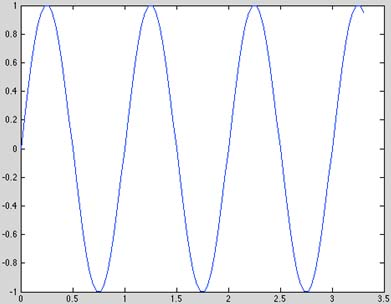
\epsfig{file=over1, scale=0.45}
      \caption{Overdrive threshold 1}
      \label{fig:over1}
    \end{center}
  \end{minipage}
  \hfill
  \begin{minipage}[t]{.45\textwidth}
    \begin{center}  
      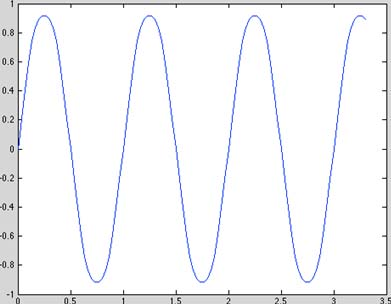
\epsfig{file=over2, scale=0.45}
      \caption{Overdrive threshold 0.5}
      \label{fig:over2}
    \end{center}
  \end{minipage}
  \hfill
\end{figure}
\subsubsection{Influence of the overdrive effect on the frequency spectrum}
To test the effects of the overdrive effect on signals, a few examples are fed into a Fast Fourier Transform (FFT) application. We test the FFT with the following signal: 
\begin{equation}
\mathrm{y(t) = 0.7 sin(2\pi \cdot 50t) + sin(2\pi \cdot 120t)}
\end{equation}
This signal combines a sinewave of frequency 50 Hz and amplitude 0.7 with a sinewave of frequency 120 Hz and amplitude 1. When the FFT is finished and plotted,figure \ref{fig:over3} below is the result.
\begin{figure}[htbp]
\centering
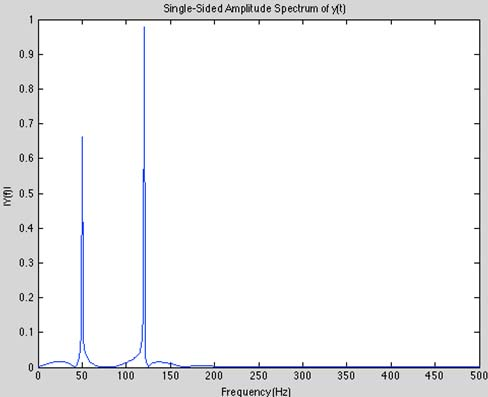
\includegraphics[height=5.5cm]{over3}
\rule{30em}{0.5pt}
\caption{FFT of a basic signal}
\label{fig:over3}
\end{figure}
The graph shown in figure \ref{fig:over4} the FFT of an overdrive with treshold equal to 0.1 on a sinewave with frequency 50hz. We can clearly see that there are only odd harmonics in the frequency spectrum, this is because the overdrive effect was set to symmetrical clipping.
%\begin{figure}[htbp]
%\centering
%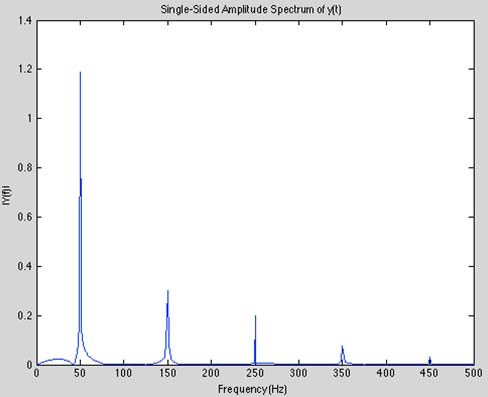
\includegraphics[height=5.5cm]{over4}
%\rule{30em}{0.5pt}
%\caption{FFT symmetric clipping}
%\label{fig:over4}
%\end{figure}
\subsubsection{Symmetrical clipping}
For a given input waveform, say a sine wave, the tops and bottoms of the waveform are clipped equally, symmetrically. For a simple sine wave, symmetrical clipping generates only odd-order harmonics, giving a reedy, or raspy sound to the resultant waveform. 
\subsubsection{Asymmetrical clipping}
The top(or bottom) of the waveform is clipped more than the bottom (top) half. This causes the generation of both even and odd harmonics, in contrast to symmetrical clipping's odd-order only. The even harmonics are smoother and more musical sounding, not as harsh as the odd ones. The hardness of the clipping and the degree of asymmetry affect the sound. The more asymmetrical, the more pronounced the even-order harmonics, the harsher the clipping, the more the harmonics are slewed toward higher orders. \\
The graph in figure \ref{fig:over5} shows the Fourier transform of a the same signal, this time overdriven using asymmetrical clipping. Here the part of the sinewave above the x-axis was clipped using the same function as in the symmetrical clipping. The part of the sinewave below the x-axis is still the original. As we can see in the graph, using the asymmetrical clipping generates not only the odd but also the even harmonics. These even harmonics give an other type of sound.
\begin{figure}[ht]
  \hfill
  \begin{minipage}[t]{.45\textwidth}
    \begin{center}  
      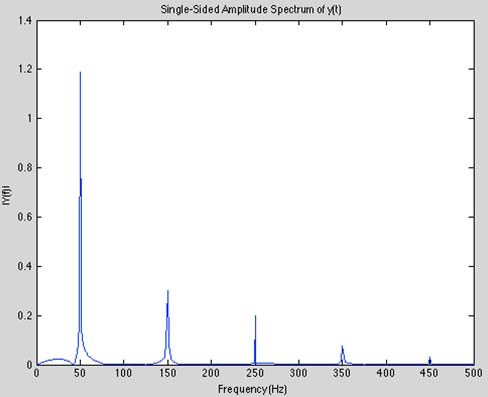
\epsfig{file=over4, scale=0.40}
      \caption{Symmetric clipping}
      \label{fig:over4}
    \end{center}
  \end{minipage}
  \hfill
  \begin{minipage}[t]{.45\textwidth}
    \begin{center}  
      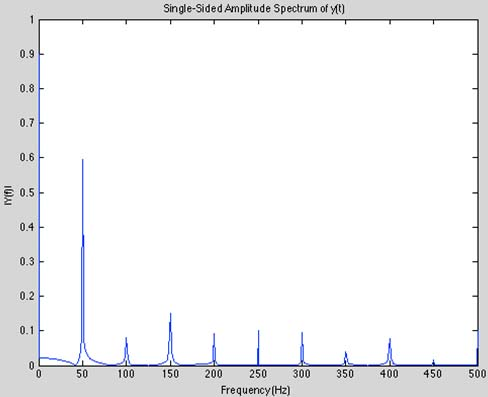
\epsfig{file=over5, scale=0.40}
      \caption{Asymmetric clipping}
      \label{fig:over5}
    \end{center}
  \end{minipage}
  \hfill
\end{figure}
%\begin{figure}[htbp]
%\centering
%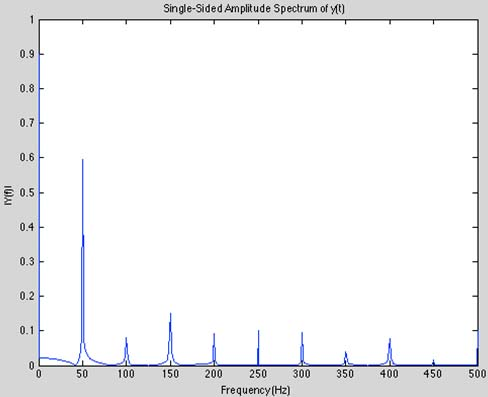
\includegraphics[height=5.5cm]{over5}
%\rule{30em}{0.5pt}
%\caption{FFT asymmetric clipping}
%\label{fig:over5}
%\end{figure}
%----------------------------------------------------------------------------------------
\section{Equaliser}
\subsection{Design of the equaliser}
The equaliser consists of three filters:
\begin{itemize}
\item Lowpass filter with cutoff frequency equal to 800Hz.
\item Bandpass filter with cutoff frequencies equal to 800Hz and 6000Hz.
\item Highpass filter with cutoff frequency equal to 6000Hz.
\end{itemize}
All the filters are constructed as FIR (Finite impulse response) with order 100. 
The filter components are created in MATLAB using the fir1 command.\\
The architecture of these Finite impulse response filters is displayed in figure \ref{fig:equal}.
\begin{figure}[htbp]
\centering
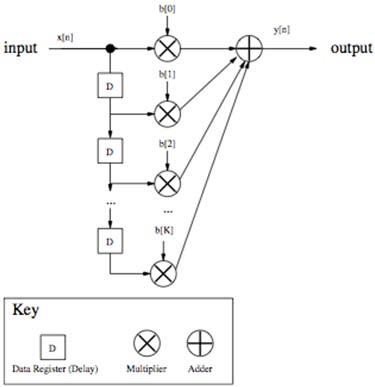
\includegraphics[height=5.5cm]{equal}
\rule{30em}{0.5pt}
\caption{Architecture of the equaliser}
\label{fig:equal}
\end{figure}
\subsection{Amplitude response of the FIR filters}
\begin{figure}[htbp]
\centering
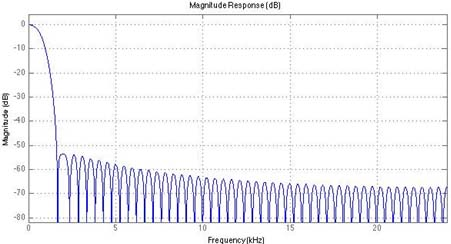
\includegraphics[height=5.5cm]{equal1}
\rule{30em}{0.5pt}
\caption{Magnitude response lowpass filter}
\label{fig:equal1}
\end{figure}
\begin{figure}[htbp]
\centering
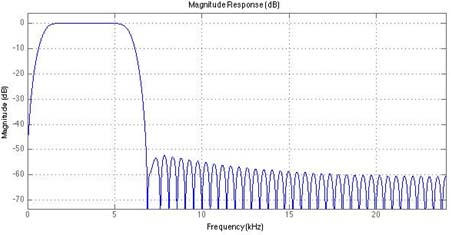
\includegraphics[height=5.5cm]{equal2}
\rule{30em}{0.5pt}
\caption{Magnitude response bandpass filter}
\label{fig:equal2}
\end{figure}
\begin{figure}[htbp]
\centering
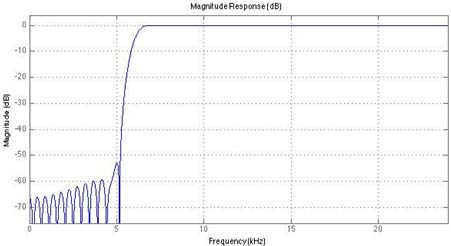
\includegraphics[height=5.5cm]{equal3}
\rule{30em}{0.5pt}
\caption{Magnitude response highpass filter}
\label{fig:equal3}
\end{figure}
%----------------------------------------------------------------------------------------
\subsection{Testing of the equalizer in MATLAB}
The equalizer has been tested by processing blocks of 1024 samples filled with white gaussian noise, the result has been fed into an FFT. Blocks are processed with the equalizer settings displayed in the caption of figures \ref{fig:equal4}, \ref{fig:equal5} and \ref{fig:equal6}.\\
\begin{figure}[htbp]
\centering
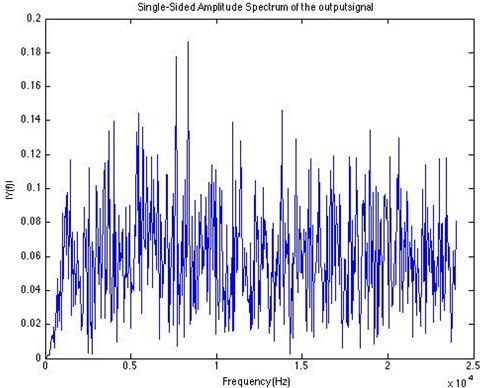
\includegraphics[height=5.5cm]{equal4}
\rule{30em}{0.5pt}
\caption{Gain$_{LP}$ = 0, Gain$_{BP}$ = 1, Gain$_{HP}$ = 1}
\label{fig:equal4}
\end{figure}
\begin{figure}[ht]
  \hfill
  \begin{minipage}[t]{.45\textwidth}
    \begin{center}  
      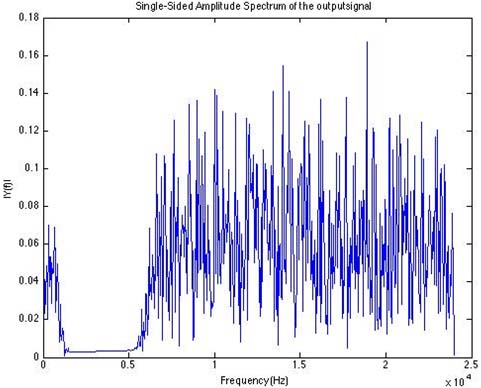
\epsfig{file=equal5, scale=0.40}
      \caption{Gain$_{LP}$ = 1, \\ Gain$_{BP}$ = 0, Gain$_{HP}$ = 1}
      \label{fig:equal5}
    \end{center}
  \end{minipage}
  \hfill
  \begin{minipage}[t]{.45\textwidth}
    \begin{center}  
      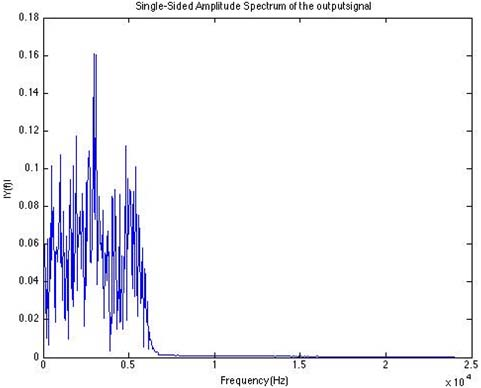
\epsfig{file=equal6, scale=0.40}
      \caption{Gain$_{LP}$ = 1, \\ Gain$_{BP}$ = 1, Gain$_{HP}$ = 0}
      \label{fig:equal6}
    \end{center}
  \end{minipage}
  \hfill
\end{figure}
The equaliser settings can be changed in the interface, using the sliders for all the filters where a value between 0 and 10 can be set. The interface will respond by sending  separate gain integers  to the dsp board. Here every filter is independently multiplied by it's gain and devided by 10. \\
Afterwards all the filter coefficients are added together to deliver the 101 final coefficients for the selected equaliser setting. These values will than be used to process the sample blocks entering the equaliser.\\
This is not the traditional way of FIR filtering, normally different coefficients are  created for every specific equalizer setting.  This way of working saves lots of processing power. \\ \\
Because the FIR filters work with samples 'from the past', every sample block will first be prepadded with the 100 last samples of the previous block.  These are stored in the so called prepad array. After the incomming block is prepadded, it 100 last samples will be stored in the prepad array. In this way always 1024 samples are loaded into the filer, this filter uses 1124 samples to create a 1024 sample outputblock. \\
%----------------------------------------------------------------------------------------
\subsection{Problems and solutions}
\begin{itemize}
\item \textbf{Problem:} The overdrive effect can only generate odd harmonics.
\begin{itemize}
\item \textbf{Solution:} An extra option is added, which lets the user choose between 'symclip' (odd harmonics) or 'asymclip' (even harmonics).
\end{itemize}
%-----------------------
\item \textbf{Problem:} The interface was not able to generate specific filter coefficients for all the different equalizer settings.
\begin{itemize}
\item \textbf{Solution:} Solved by designing a filtering method which can use 'static' coefficients. Here the interface only has to send the different gain integers to the dsp board.
\end{itemize}
%-----------------------
\item \textbf{Problem:} The FIR filter goes back 100 samples in the past to proces the current sample. 
\begin{itemize}
\item \textbf{Solution:} An extra 'prepad' array is added, initiated by zeros when the equalizer starts, and always saves the last 100 samples of the 1024 sample block. Allowing the filter to use these samples.
\end{itemize}
%-----------------------
\item \textbf{Problem:} The filter coefficients for the highpass filter are to large for the 32-bit double values, the dsp board uses.
\begin{itemize}
\item \textbf{Solution:} We first changed the compiler settings to use 64-bit memory for the values, but this caused the rest of the program to stop working. It was finally solved by creating new filter coefficients for the high pass filter who where small enough to fit in 32 bits.
\end{itemize}
%-----------------------
\item \textbf{Problem:} The equalizer added an extra noise to the signal
\begin{itemize}
\item \textbf{Solution:} The problem here was that the prepad array was not filled correctly, so it prepadded every sample block with 100 zeros as it was initiated. The last 100 samples where always saved in a wrong place in the memory. The use of pointers for this storing and fetching caused the program not to crash during runtime. Correcting the save location solved this.
\end{itemize}
\item \textbf{Problem:} The bandpass filter acts as a highpass from its first cutoff frequency
\begin{itemize}
\item \textbf{Solution:} at implement
\end{itemize}
\end{itemize}
